
% \clearpage
\subsection{ออกแบบแบบจำลองของหุ่นยนต์ฮิวมานอยด์ UTHAI}
การออกแบบนี้มีเป้าหมายเพื่อ สร้างแบบจำลองของหุ่นยนต์ฮิวมานอยด์ UTHAIให้ถูกต้องตามที่โครงสร้างทางกลได้สร้างเอาไว้
โดยใช้โปรแกรม RViz เป็นตัวแสดงผลให้เห็นเป็นภาพ
\begin{figure}[!ht]
    \centering
    \begin{subfigure}[b]{0.4\textwidth}
        \centering
        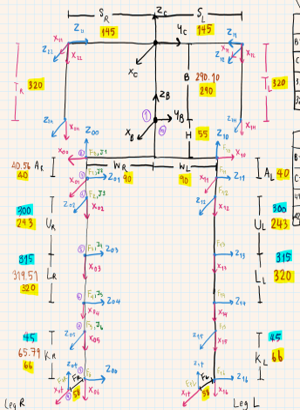
\includegraphics[width=\textwidth]{chapter3/images/uthai_sk.png}
        \caption{ค่าพารามิเตอร์ที่ใช้ในการสร้างแบบจำลอง}
    \end{subfigure}
    \hfill
    \begin{subfigure}[b]{0.5\textwidth}
        \centering
        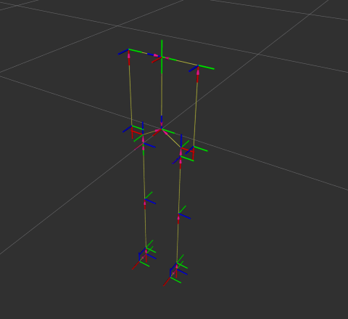
\includegraphics[width=\textwidth]{chapter4/images/urdf_rviz0.png}
        \caption{URDF ที่มีแต่โครงไม่มีก้านต่อ}
    \end{subfigure}
    \caption{URDF ที่แสดงผลใน RViz}
\end{figure}
% \begin{figure}[!ht]
% 	\centering
% 	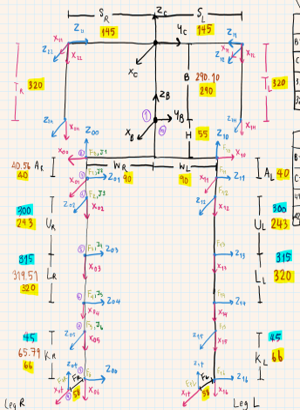
\includegraphics[width=0.5\textwidth]{chapter3/images/uthai_sk.png}
% 	\caption{ค่าพารามิเตอร์ที่ใช้ในการสร้างแบบจำลอง}
% \end{figure}
% \begin{figure}[!ht]
% 	\centering
% 	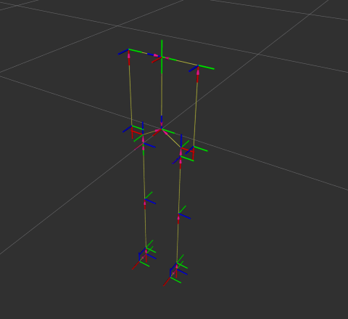
\includegraphics[width=\textwidth]{chapter4/images/urdf_rviz0.png}
% 	\caption{URDF ที่มีแต่โครงไม่มีก้านต่อ}
% \end{figure}
\begin{figure}[!ht]
    \centering
    \begin{subfigure}[b]{0.3\textwidth}
        \centering
        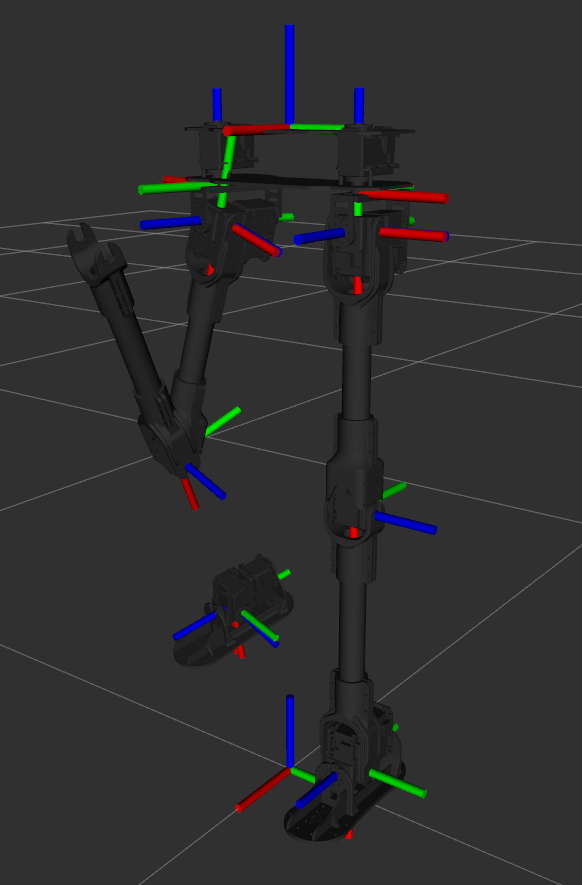
\includegraphics[width=\textwidth]{chapter4/images/urdf_rviz1.png}
        \caption{URDF ที่เกิดข้อผิดพลาด}
    \end{subfigure}
    \hfill
    \begin{subfigure}[b]{0.5\textwidth}
        \centering
        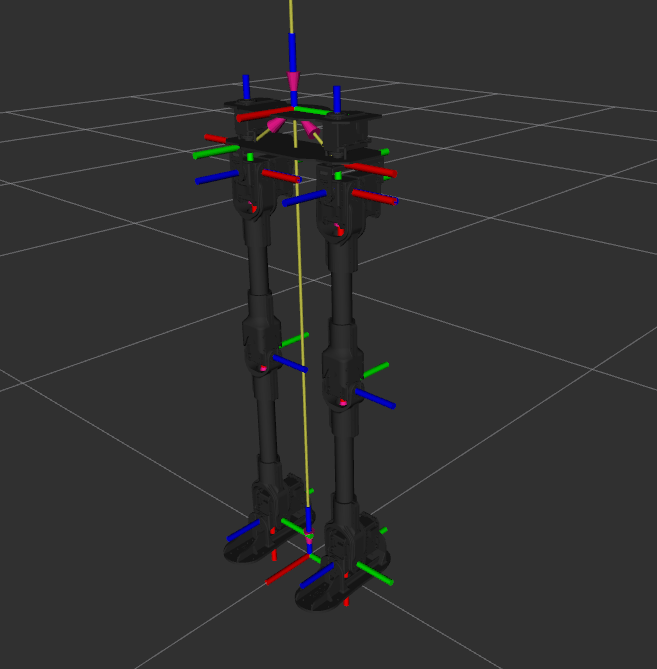
\includegraphics[width=\textwidth]{chapter4/images/urdf_rviz2.png}
        \caption{URDF ที่ทำงานได้ถูกต้อง}
    \end{subfigure}
    \caption{URDF ที่แสดงผลใน RViz}
\end{figure}

\clearpage
\subsection{การสั่งงานข้อต่อใน RViz ผ่าน GUI}
การเขียนโปแกรมในส่วนนี้มีเป้าหมายเพื่อ ทดสอบการทำงานของโปรแกรม RViz ที่จะแสดงการทำงานของข้อต่อเป็นอย่างไร
การวางเฟรมของหุ่นยนต์นั้นมีความถูกต้องหรือไม่
\begin{figure}[!ht]
	\centering
	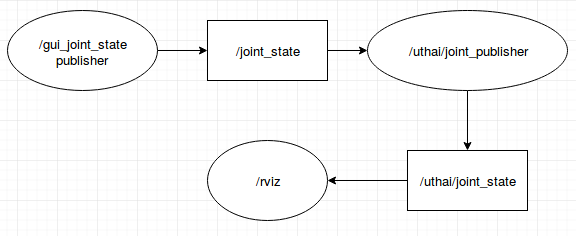
\includegraphics[width=0.9\textwidth]{chapter3/images/uthai_joint_gui.png}
	\caption{การสั่งการข้อต่อใน RViz ผ่าน GUI}
\end{figure}

หลังจากที่ทำการทดลองเสร็จแล้วพบว่าสิ่งที่ขาดหายไปคือการตั้งค่า Joint limit ให้กับหุ่นยนต์ฮิวมานอยด์ในโปรแกรม RViz
จึงต้องกลับไปแก้ค่าและทดสอบใหม่ จากนั้นถือว่าการทดลองเสร็จสิ้น สามารถที่จะควบคุมการเคลื่อนไหวของแต่ละข้อต่อผ่าน GUI ได้

\begin{figure}[!ht]
    \centering
    \begin{subfigure}[b]{0.15\textwidth}
        \centering
        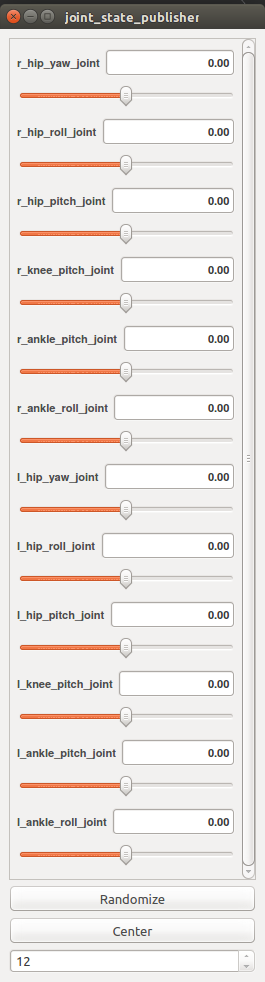
\includegraphics[width=\textwidth]{chapter4/images/uthai_rviz_gui.png}
        \caption{GUI สำหรับสั่งงานแต่ละข้อต่อ}
    \end{subfigure}
    \hfill
    \begin{subfigure}[b]{0.50\textwidth}
        \centering
        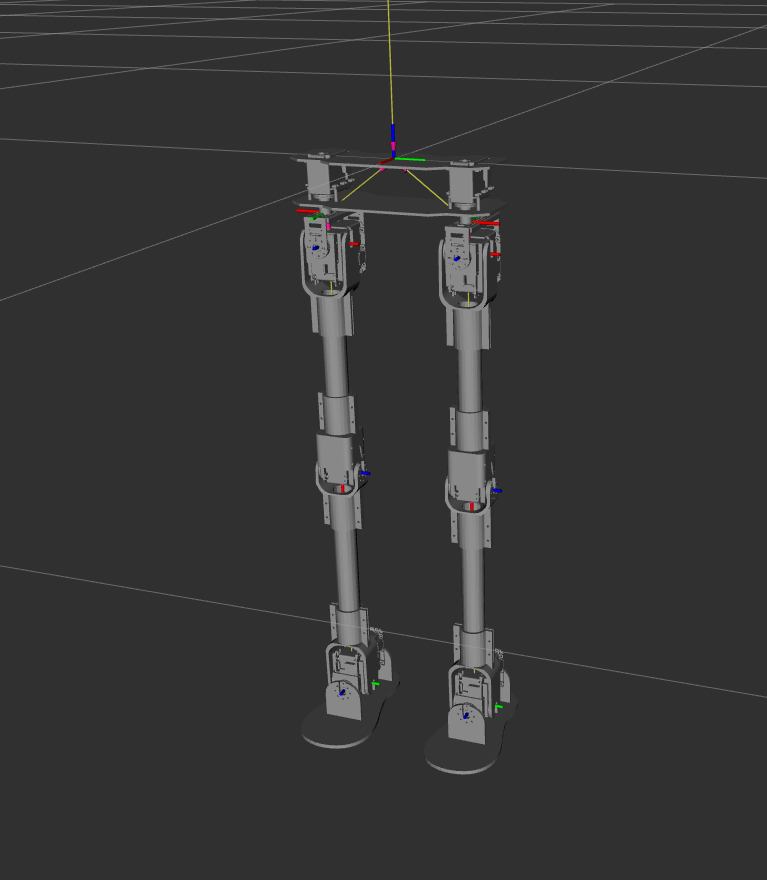
\includegraphics[width=\textwidth]{chapter4/images/uthai_rviz_model.png}
        \caption{หุ่นยนต์ที่แสดงผลในโปรแกรม RViz}
    \end{subfigure}
    \caption{การสั่งการข้อต่อใน RViz ผ่าน GUI}
\end{figure}


\clearpage
\subsection{การเขียนโปรแกรมอ่านตำแหน่งจากเซอร์โวมอเตอร์เข้าระบบ}
การเขียนโปรแกรมในส่วนนี้มีเป้าหมายเพื่อ ทดสอบการอ่านตำแหน่งจากเซอร์โวมอเตอร์
และทดสอบการสั่งการระบบแสดงผลด้วยภาพ จึงได้ออกแบบการทดลองนี้ขึ้นมา
การดำเนินการเริ่มจาก เขียนโปรแกรมสำหรับอ่านค่าตำแหน่งจากเซอร์โวซึ่งจะได้ตำแหน่งออกมาใน topic
JointState หลังจากนั้นก็จึงแปลงให้อยู่ใน message เดียวกับที่ Rviz ต้องการ แล้วจึงสั่งออกไป
\begin{figure}[!ht]
	\centering
	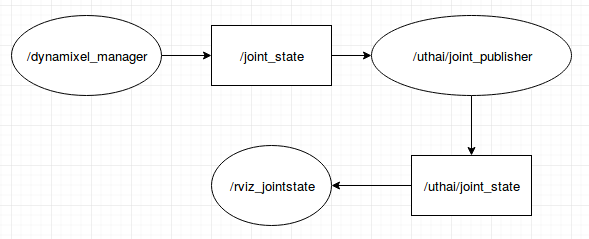
\includegraphics[width=0.8\textwidth]{chapter3/images/rviz_joint_state.png}
	\caption{การติดต่อสื่อสารระหว่างจากเซอร์โวมอเตอร์กับระบบ}
\end{figure}
% \clearpage
\begin{figure}[!ht]
    \centering
    \begin{subfigure}[b]{0.45\textwidth}
        \centering
        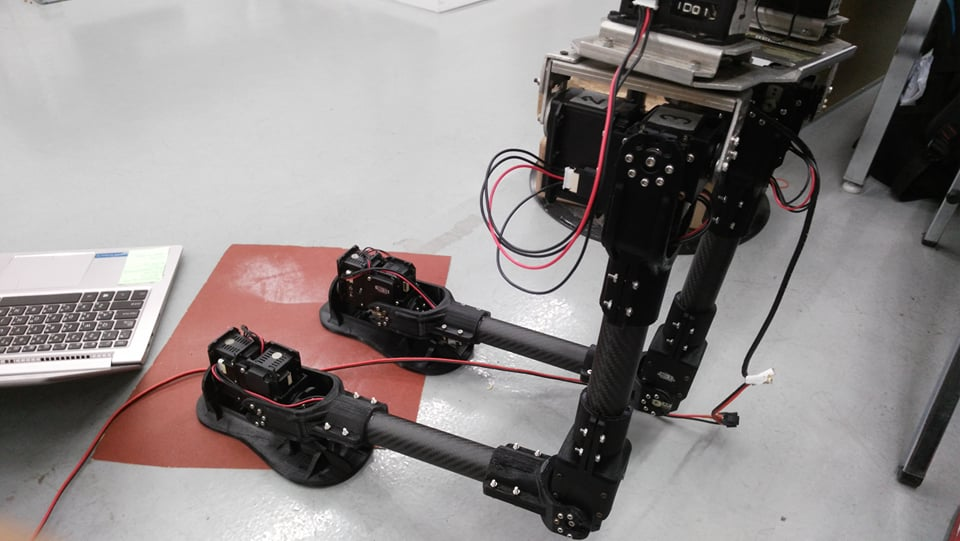
\includegraphics[width=\textwidth]{chapter4/images/robot_2_rviz1.jpg}
        \caption{หุ่นยนต์ตัวจริง}
    \end{subfigure}
    \hfill
    \begin{subfigure}[b]{0.45\textwidth}
        \centering
        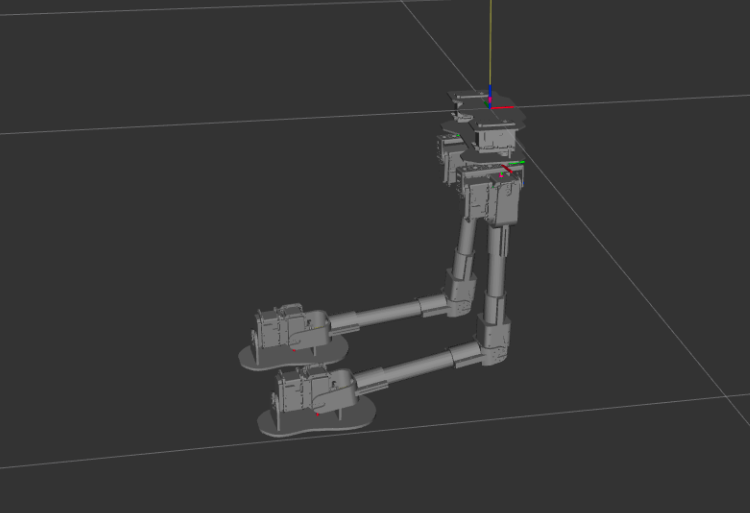
\includegraphics[width=\textwidth]{chapter4/images/robot_2_rviz1.png}
        \caption{หุ่นยนต์ใน RViz}
    \end{subfigure}
    \caption{การแสดงผลท่าทาง 1}
	\label{fig:robot_2_rviz1}
\end{figure}
\begin{figure}[!ht]
    \centering
    \begin{subfigure}[b]{0.45\textwidth}
        \centering
        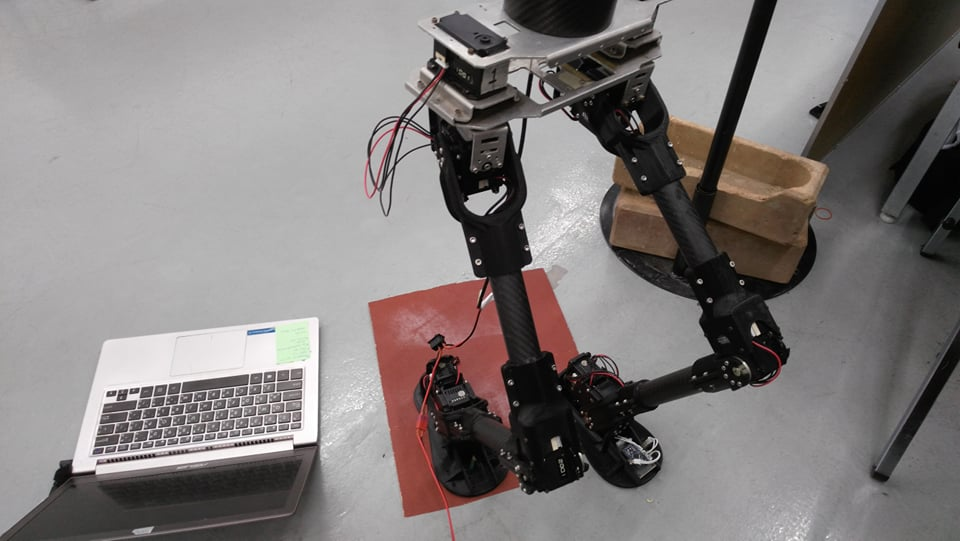
\includegraphics[width=\textwidth]{chapter4/images/robot_2_rviz2.jpg}
        \caption{หุ่นยนต์ตัวจริง}
    \end{subfigure}
    \hfill
    \begin{subfigure}[b]{0.32\textwidth}
        \centering
        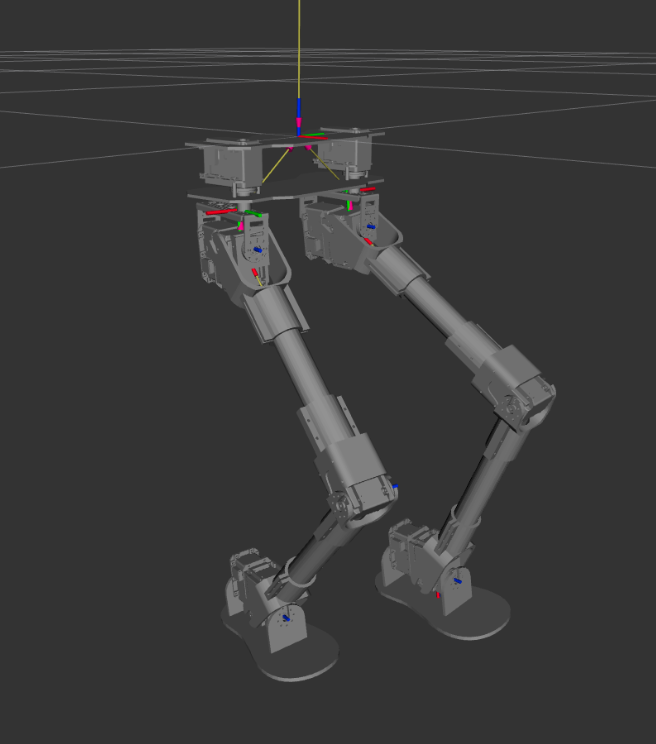
\includegraphics[width=\textwidth]{chapter4/images/robot_2_rviz2.png}
        \caption{หุ่นยนต์ใน RViz}
    \end{subfigure}
    \caption{การแสดงผลท่าทาง 2}
	\label{fig:robot_2_rviz2}
\end{figure}


\clearpage
\begin{figure}[!ht]
    \centering
    \begin{subfigure}[b]{0.45\textwidth}
        \centering
        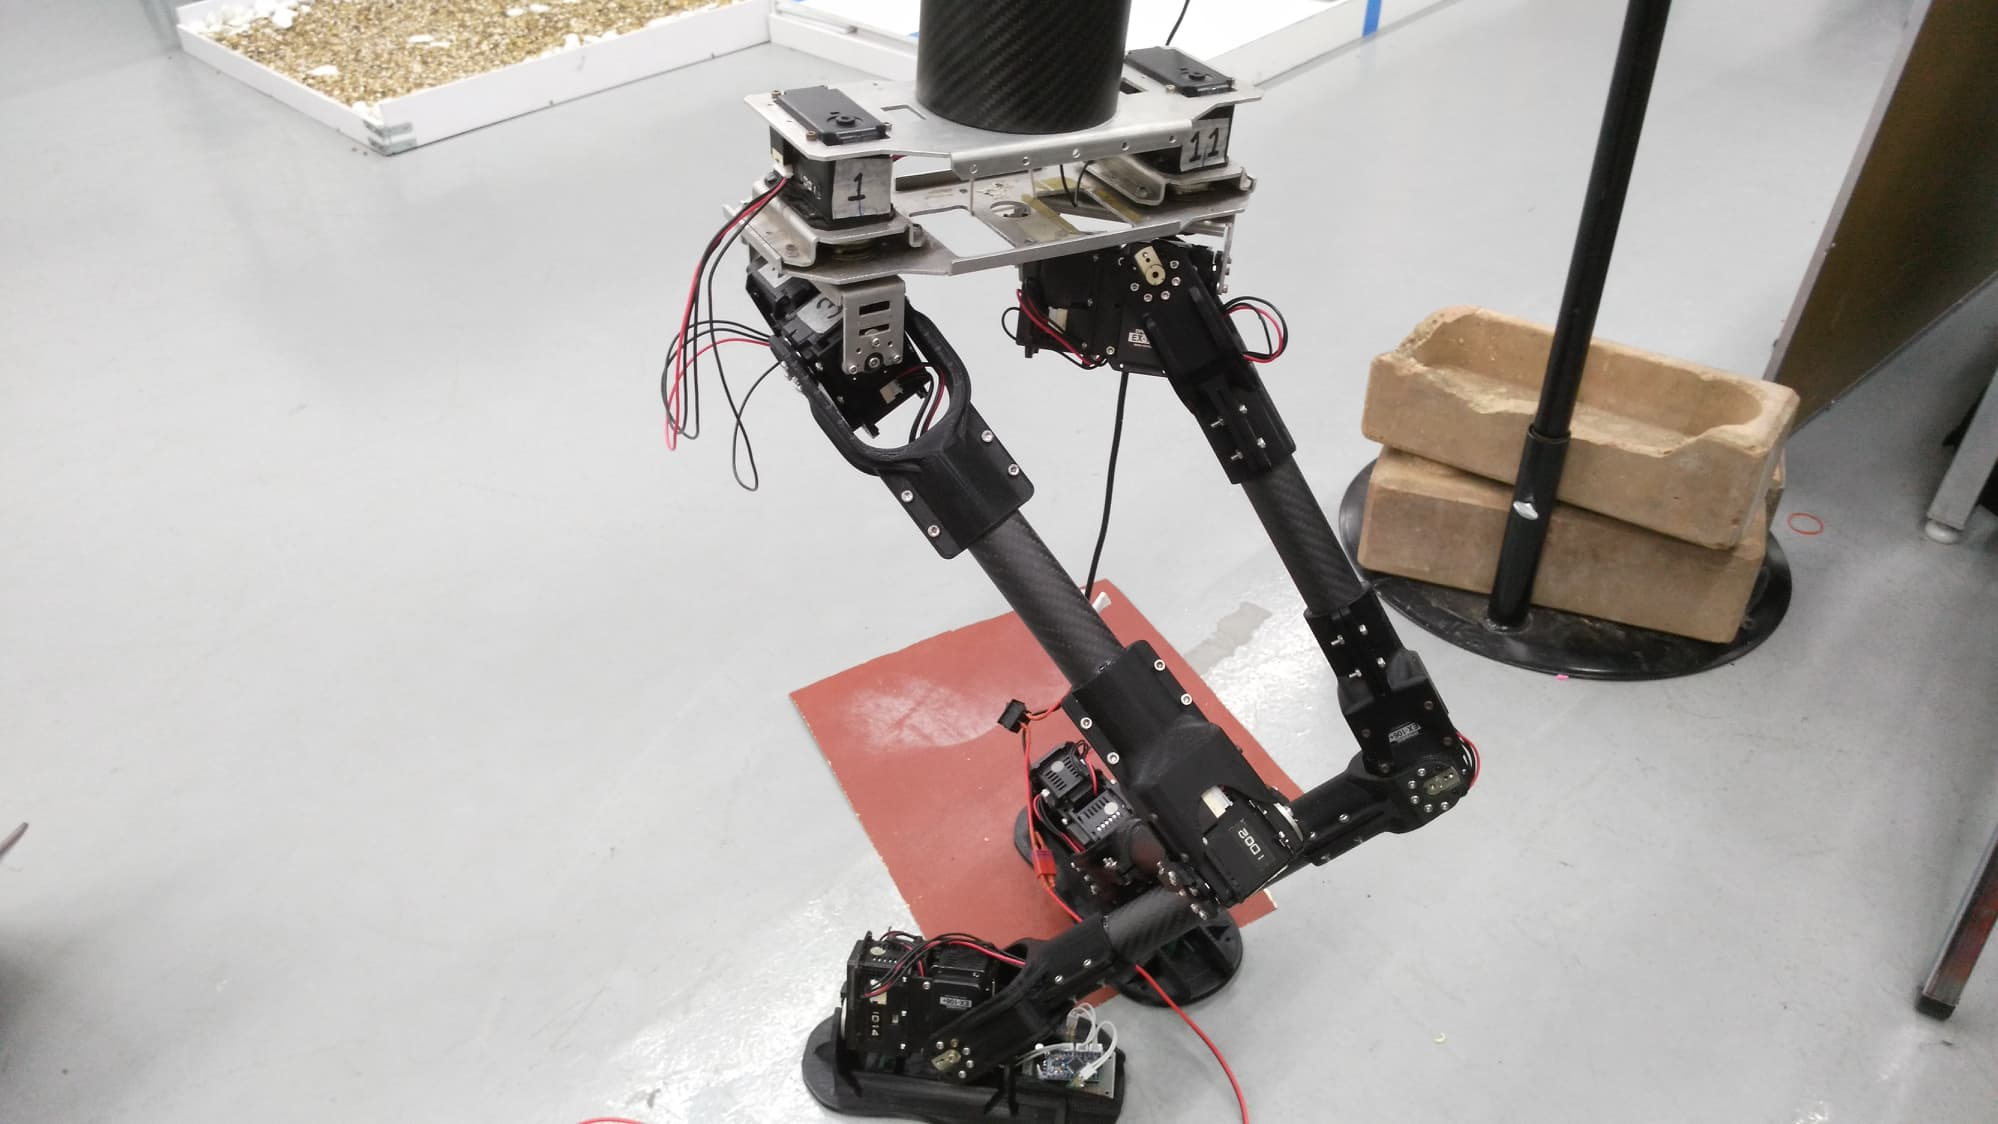
\includegraphics[width=\textwidth]{chapter4/images/robot_2_rviz3.jpg}
        \caption{หุ่นยนต์ตัวจริง}
    \end{subfigure}
    \hfill
    \begin{subfigure}[b]{0.35\textwidth}
        \centering
        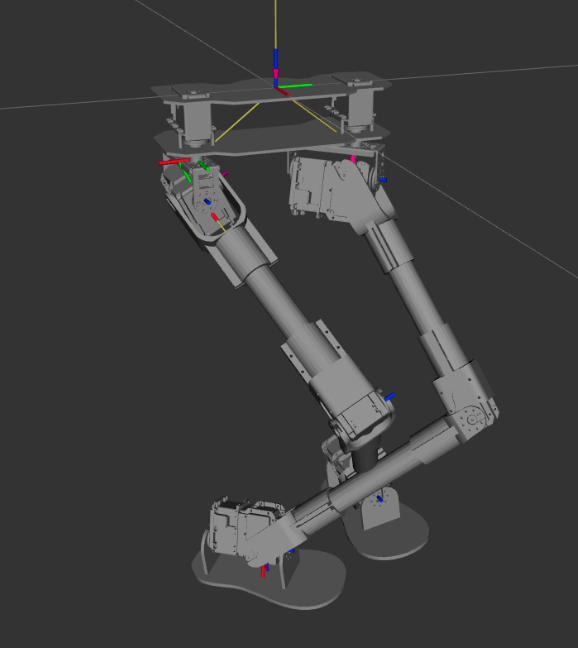
\includegraphics[width=\textwidth]{chapter4/images/robot_2_rviz3.png}
        \caption{หุ่นยนต์ใน RViz}
    \end{subfigure}
    \caption{การแสดงผลท่าทาง 3}
	\label{fig:robot_2_rviz3}
\end{figure}

\subsection{การส่งตำแหน่งของเซอร์โวมอเตอร์ไปประมวลผลหาจุดศูนย์กลางมวล}
การเขียนโปรแกรมในส่วนนี้มีเป้าหมายเพื่อ ทดสอบการทำงานการเชื่อมต่อกับโปรแกรมภายนอกโดยการส่งค่าตำแหน่งของเซอร์โวมอเตอร์
ออกไปแล้วมีโปรแกรมจาก MATLAB รับตำแหน่งไปแล้วประมวลผลเพื่อเอาตำแหน่งของจุดศูนย์รวมมวลเข้ามาแสดงในโปรแกรม Rviz
\begin{figure}[!ht]
	\centering
	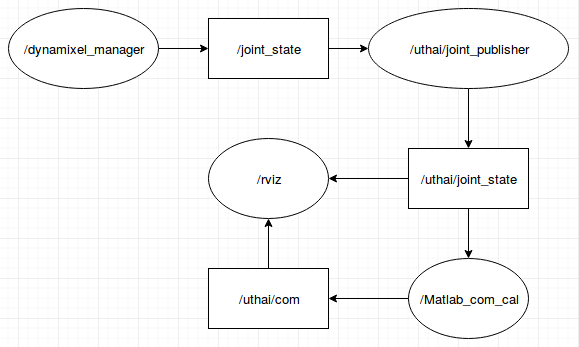
\includegraphics[width=0.9\textwidth]{chapter3/images/matlab_com.png}
	\caption{การประมวลผลตำแหน่งจุดศูนย์กลางมวลด้วย MATLAB}
\end{figure}

\begin{figure}[!ht]
	\centering
	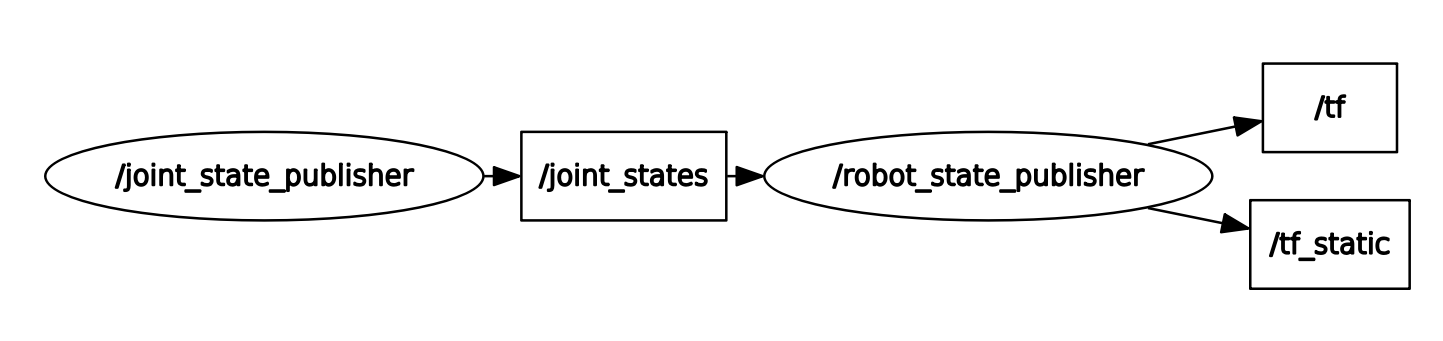
\includegraphics[width=\textwidth]{chapter4/images/com_uthai_node0.png}
	\caption{การเชื่อมต่อกันระหว่าง Node ก่อนเชื่อมต่อเซอร์โวมอเตอร์}
\end{figure}
\begin{figure}[!ht]
	\centering
	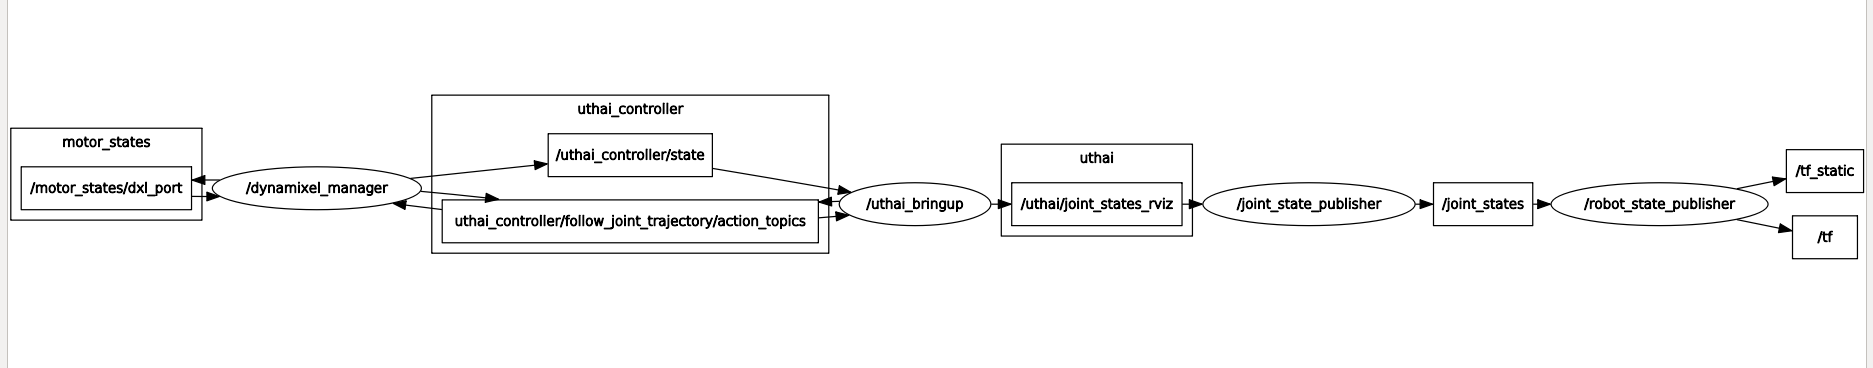
\includegraphics[width=\textwidth]{chapter4/images/com_uthai_node.png}
	\caption{การเชื่อมต่อกันระหว่าง Node หลังเชื่อมต่อเซอร์โวมอเตอร์}
\end{figure}
\begin{figure}[!ht]
	\centering
	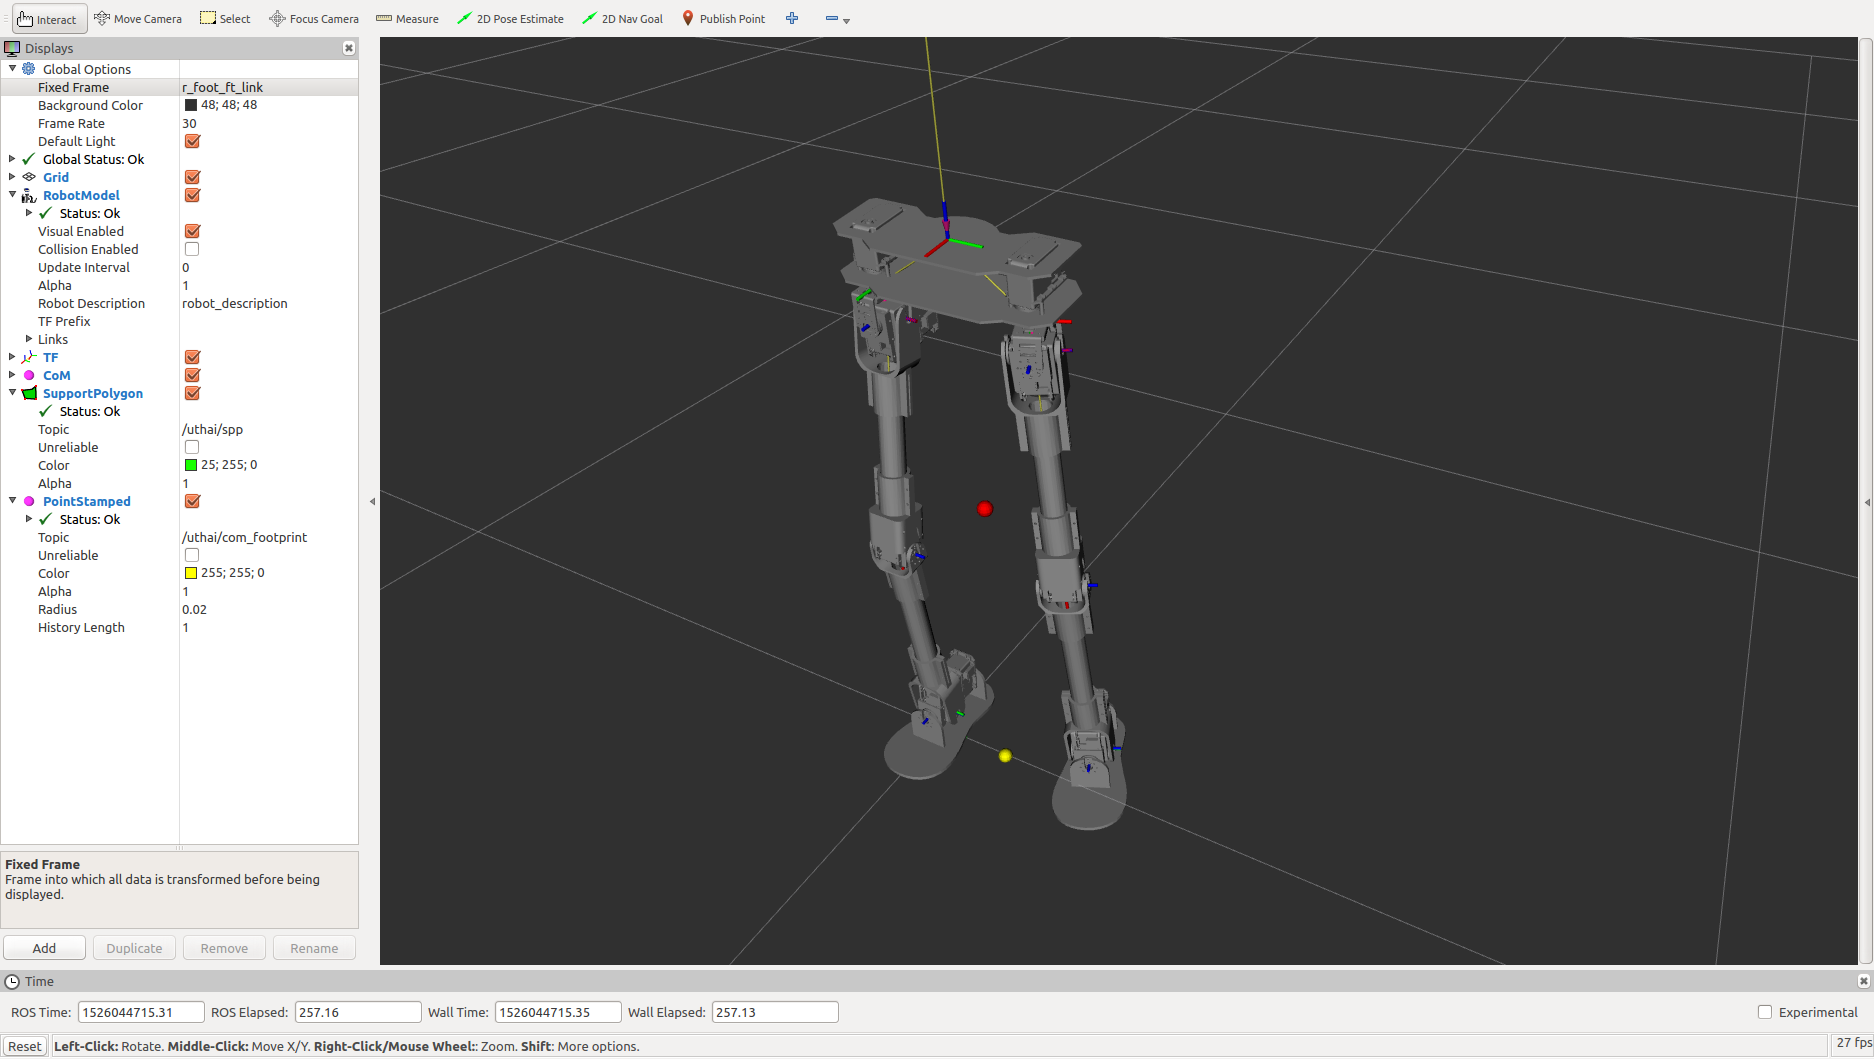
\includegraphics[width=\textwidth]{chapter4/images/com_uthai.png}
	\caption{การประมวลผลตำแหน่งหาจุดศูนย์กลางด้วย MATLAB}
\end{figure}

%%%%%%%%%%%%%%%%%%%%%%%%%%%%%%%%%%%%%%%%%%%%%%%%%%%%%%%%%%%%%%%%%%%%%%%%%%%%%%%
\clearpage
\subsection{การเขียนโปรแกรมเซนเซอร์ตรวจจับการสัมผัสพื้น}
การเขียนโปรแกรมในส่วนนี้มีเป้าหมายเพื่อ บอกให้ตัวประมวลผลระดับสูงรับรู้ว่าเท้าฝั่งไหนมีการสัมผัสกับพื้น
เพื่อใช้ในการเปลี่ยนสถานะของโปรแกรมในการคำนวณ ตัวเซนเซอร์ตรวจจับฝ่าเท้านั้นใช้เป็น Arduino Pro-Mini
เนื่องจากมีขนาดเล็กและสามารถเชื่อมต่อกับเซนเซอร์วัดแรงกดได้สูงสุด 6 ตัว เมื่อได้ไอเดียแล้วจากนั้นจึงวางโฟลชาร์ต
การทำงานของโปรแกรม เมื่อได้โฟลชาร์ตแล้วจึงเริ่มเขียนโปรแกรมเพื่อทดสอบการทำงาน

\begin{figure}[!ht]
    \centering
    \begin{subfigure}[b]{0.40\textwidth}
        \centering
        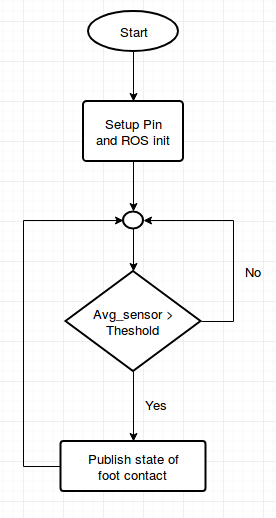
\includegraphics[width=\textwidth]{chapter3/images/gcs_flowchart.png}
        \caption{โฟลชาร์ตของเซนเซอร์ตรวจจับพื้น}
    \end{subfigure}
    \hfill
    \begin{subfigure}[b]{0.50\textwidth}
        \centering
        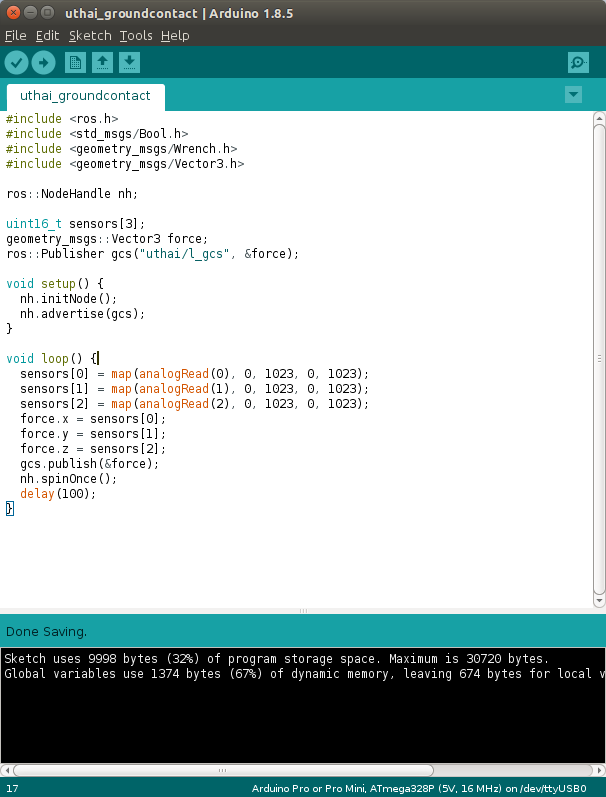
\includegraphics[width=\textwidth]{chapter3/images/code_arduino_uthai.png}
        \caption{โปรแกรมของเซนเซอร์ตรวจจับพื้น}
    \end{subfigure}
    \caption{เซนเซอร์ตรวจจับพื้น}
\end{figure}

\begin{figure}[!ht]
	\centering
	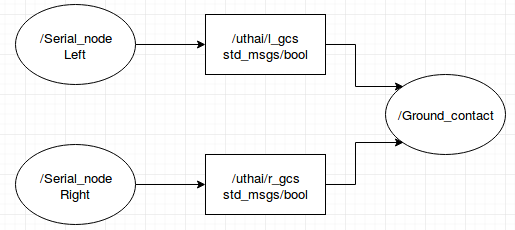
\includegraphics[width=0.8\textwidth]{chapter3/images/node_gcs.png}
	\caption{การติดต่อสื่อสารระหว่างจากเซนเซอร์ตรวจจับเท้ากับระบบ}
\end{figure}




